%%%%%%%%%%%%%%%%%%%%%%%%%%%%%%%%%%%%%%%%%%%%%%%%%%%
%% Manual completo del vehículo UAL-eCARM           	                      %%
%% Author:  Francisco José Mañas Álvarez                                        %%
%%%%%%%%%%%%%%%%%%%%%%%%%%%%%%%%%%%%%%%%%%%%%%%%%%%
\documentclass[11pt,a4paper,openright,twoside,final]{book}
%%%%%%%%%%%%%%%%%%%%%%%%%%%%%%%%%%%%%%%%%%%%%%
% PAQUETES
%%%%%%%%%%%%%%%%%%%%%%%%%%%%%%%%%%%%%%%%%%%%%%
\usepackage[T1]{fontenc}
\usepackage[spanish,activeacute] {babel}
\usepackage[utf8]{inputenc}
\usepackage{lmodern} \normalfont %to load T1lmr.fd 

\usepackage{hyperref}
\usepackage{float}
\usepackage{amssymb,amsmath,amsbsy} % símbolo
\usepackage{upgreek} % para poner letras griegas sin cursiva
\usepackage{cancel}
\usepackage{cite}
\usepackage{mathdots} % para el comando \iddots
\usepackage{mathrsfs} % para formato de letra
\usepackage{stackrel} % para el comando \stackbin
\usepackage{graphicx}
\usepackage{subfig}
\usepackage{tabulary}
\usepackage{booktabs}
\usepackage{setspace}
\usepackage{vmargin}
\usepackage{enumitem}
\usepackage{acronym}
\usepackage{url}
\usepackage{pdfpages}
\usepackage{multirow}
\usepackage{bookmark}
\usepackage[toc,page, title, titletoc]{appendix}
\usepackage{blindtext}
\usepackage[labelsep=period]{caption}
\usepackage{listings} % Para el código 
%%%%%%%%%%%%%%%%%%%%%%%%%%%%%%%%%%%%%%%%%%%%%%
% FORMATO
%%%%%%%%%%%%%%%%%%%%%%%%%%%%%%%%%%%%%%%%%%%%%%
% MARGENES
\setmargins	{2.5cm}       % margen izquierdo
			{2.5cm}       % margen superior
			{16.0cm}      % anchura del texto
			{22.2cm}      % altura del texto
			{14.16pt}     % altura de los encabezados
			{1cm}         % espacio entre el texto y los encabezados
			{14.16pt}     % altura del pie de página
			{1cm}         % espacio entre el texto y el pie de página
% CABECERA Y PIE DE PÁGINA
\usepackage{fancyhdr}
\pagestyle{fancy}
\fancyhead[L,C,R,LO]{}
\renewcommand{\headrulewidth}{0.5pt}
\renewcommand{\footrulewidth}{0.5pt}
\fancyhead[RO]{\leftmark}
\fancyhead[LE]{\rightmark}
\fancyhead[RE]{Grupo A.R.M. TEP-197}
\fancyfoot[LE,RO]{\thepage}
\fancyfoot[RE,LO]{UAL-eCARM}
\fancyfoot[C]{}

\fancypagestyle{normal}{
\renewcommand{\headrulewidth}{0.5pt}
\renewcommand{\footrulewidth}{0.5pt}
\fancyhead[LO,RO,LE,RE,C]{}
\fancyfoot[LE,RO]{\thepage}
\fancyfoot[RE,LO]{UAL-eCARM}
}
% Encabezados y pies de página.
\fancypagestyle{plain}{
	\fancyhead[L,C,R]{}
	\fancyfoot[C]{}
	\fancyfoot[L]{UAL-eCARM}
	\fancyfoot[R]{\thepage}
	\renewcommand{\headrulewidth}{0pt}
	\renewcommand{\footrulewidth}{0.5pt}
}
% Estilo creado
\fancypagestyle{blanco}{%
\fancyhead{}
\fancyfoot{}
\renewcommand{\headrulewidth}{0pt}
\renewcommand{\footrulewidth}{0pt}
}
\usepackage{afterpage}
\newcommand\blankpage{
    \null
    \thispagestyle{empty}
    \newpage}

% PORTADA
\title{\Huge \textbf{UAL-eCARM} \\ \huge Manual descriptivo completo}
% Author
\author{\textsc{Grupo de Automática, Robótica y Mecatrónica (ARM).}}

\begin{document}
\frontmatter
\renewcommand{\tablename}{Tabla}
\renewcommand{\listtablename}{Índice de tablas}
\maketitle
\afterpage{\blankpage}

% INDICES
\tableofcontents
\afterpage{\blankpage}
\listoffigures
\afterpage{\blankpage}
\listoftables
\afterpage{\blankpage}
\mainmatter

% Capítulo 1. Introducción
%%%%%%%%%%%%%%%%%%%%%%%%%%%%%%%%%%%%%%%%%%%%%%
% Capítulo de introducción
%%%%%%%%%%%%%%%%%%%%%%%%%%%%%%%%%%%%%%%%%%%%%%
\chapter{Introducción}
\section{El vehículo}
El vehículo eléctrico que posee la Universidad de Almería (UAL) se muestra en la Figura \ref{fig:vehiculo}. Este vehículo fue adquirido en el año 2010 a la empresa Tesur, equipado inicialmente por dicha empresa con los componentes necesarios para el correcto funcionamiento de la propulsión y la dirección asistida del vehículo. Todo este equipamiento es denominado \textit{Caja Tesur} y con el paso del tiempo y los distintos desarrollos llevados a cabo sobre el vehículo se ha sustituido por diferentes componentes. 

\begin{figure}[!ht]
  \centering
    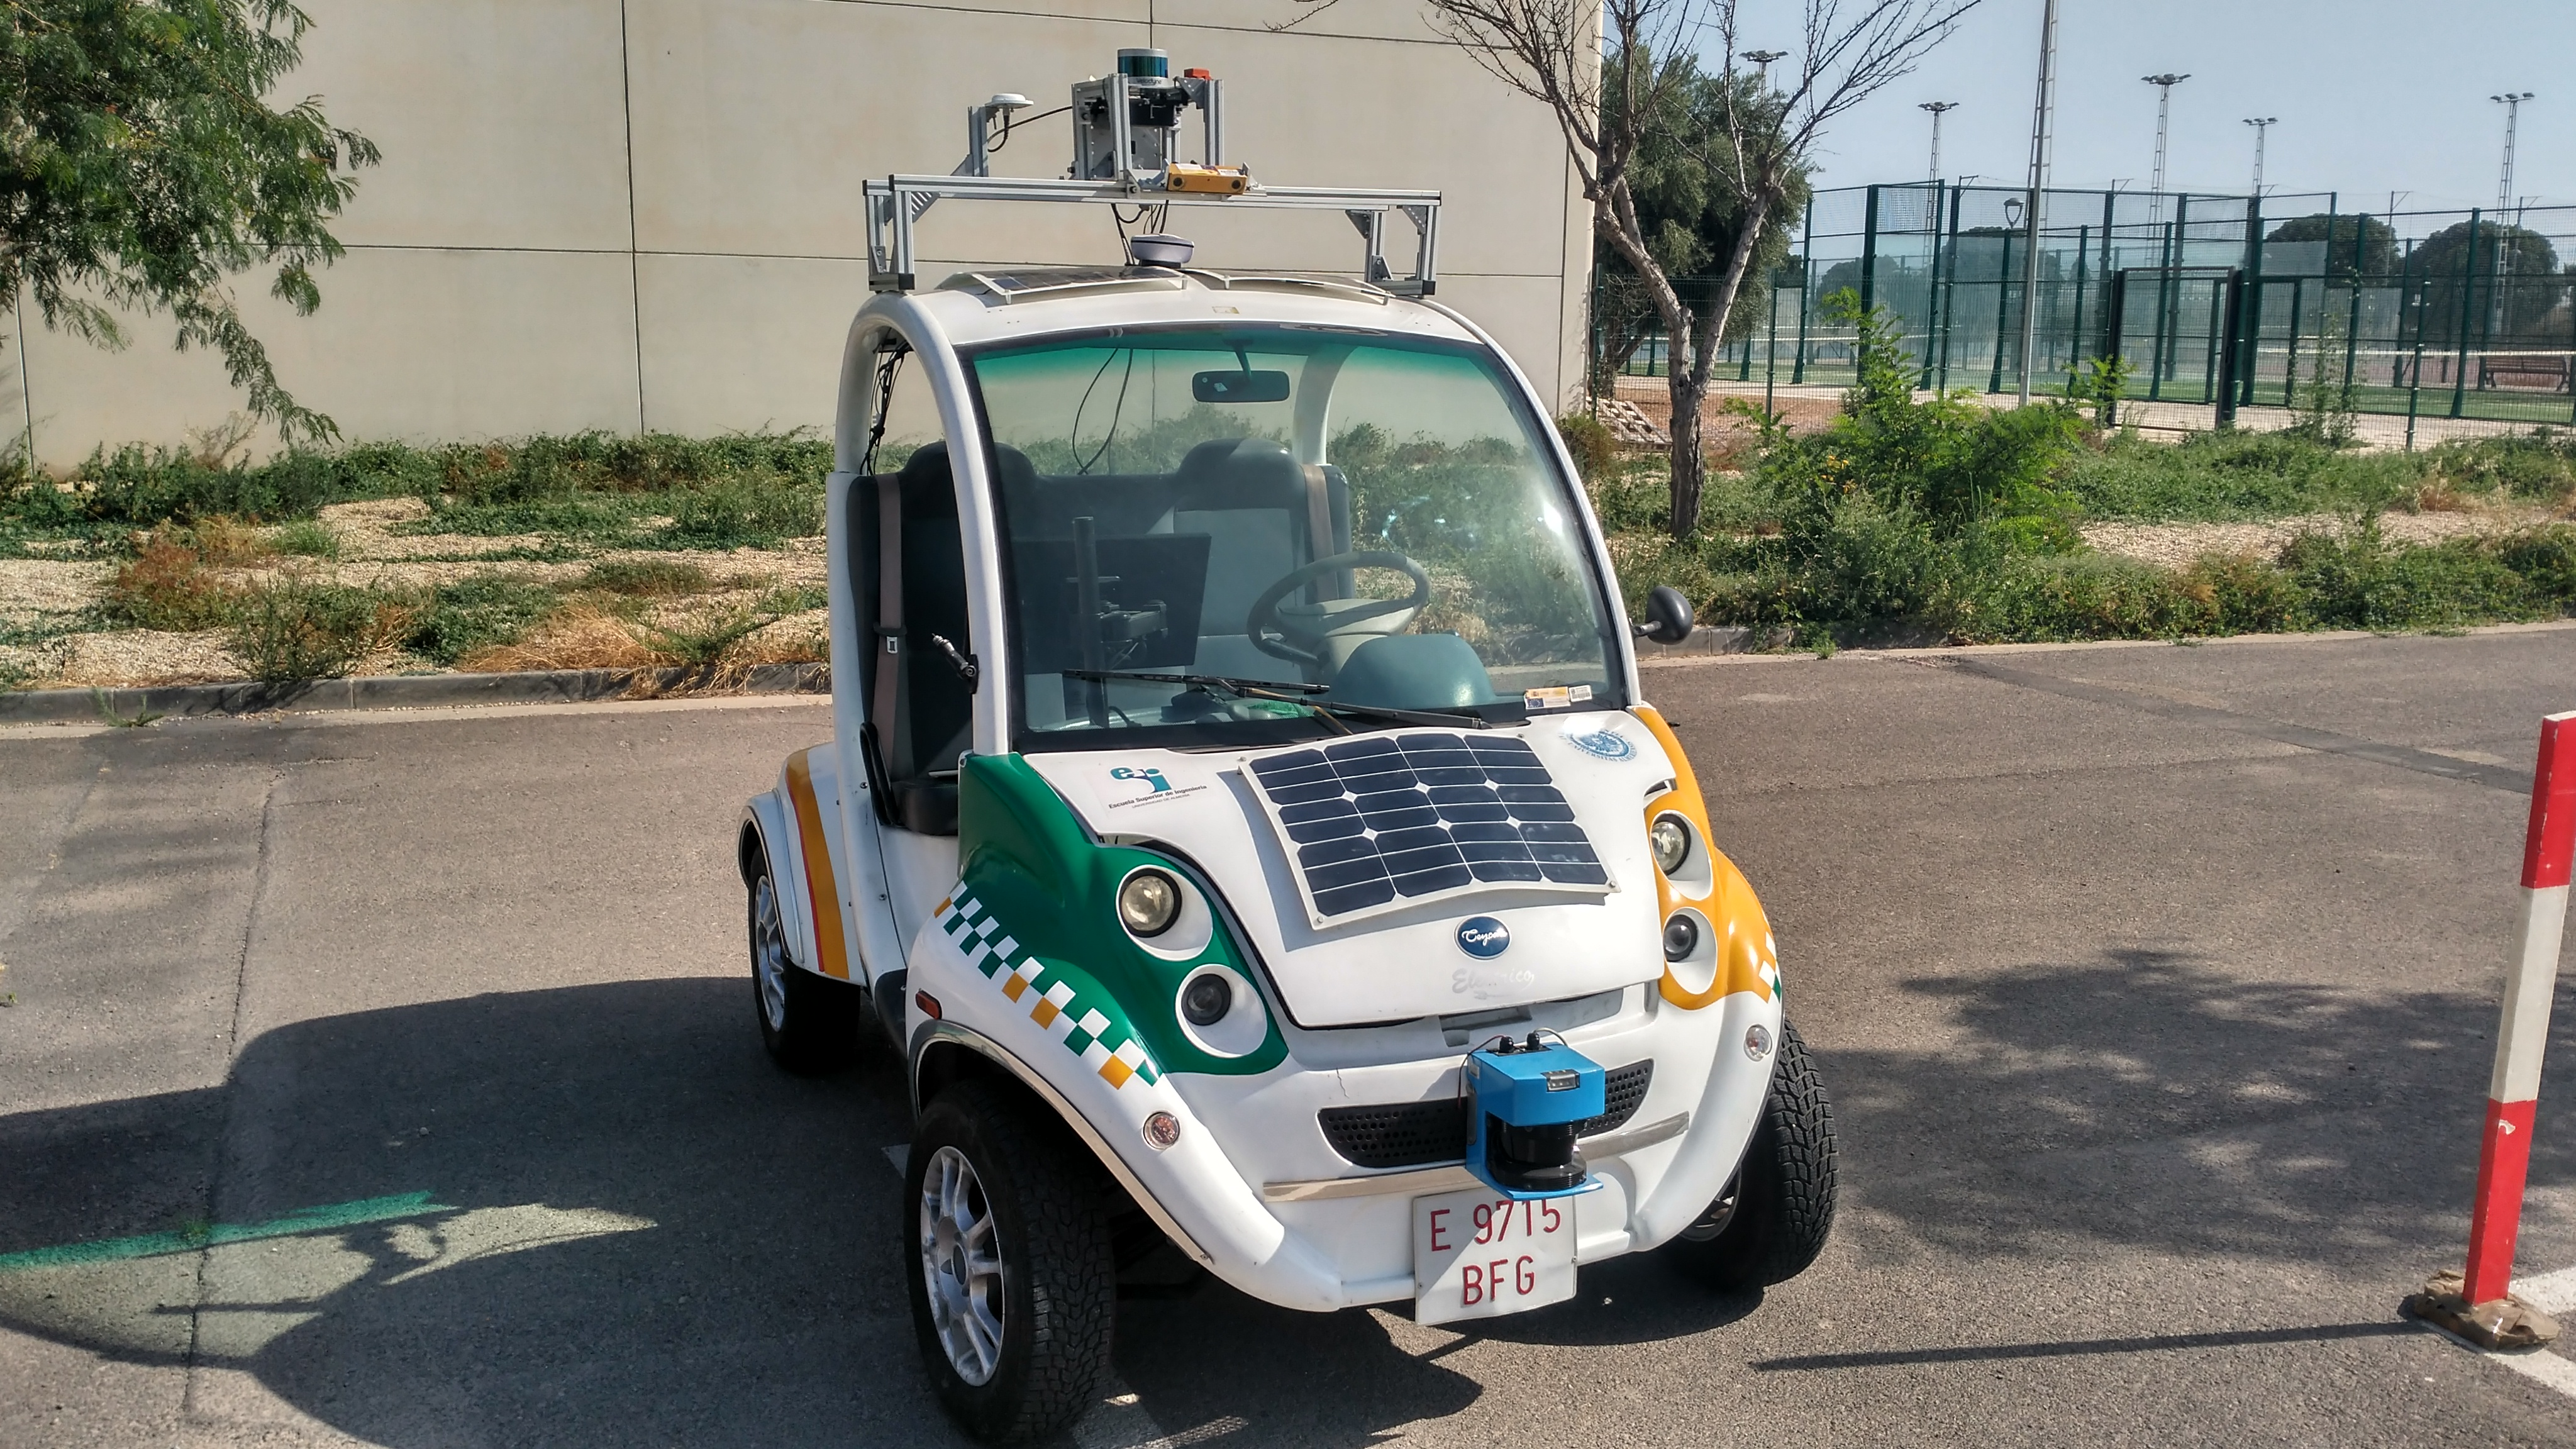
\includegraphics[width=1\textwidth]{Figuras/vehiculo-aparcamientos.jpg}
  \caption{Vehículo UAL-eCARM.}
  \label{fig:vehiculo}
\end{figure}

\begin{figure}[!ht]
  \centering
    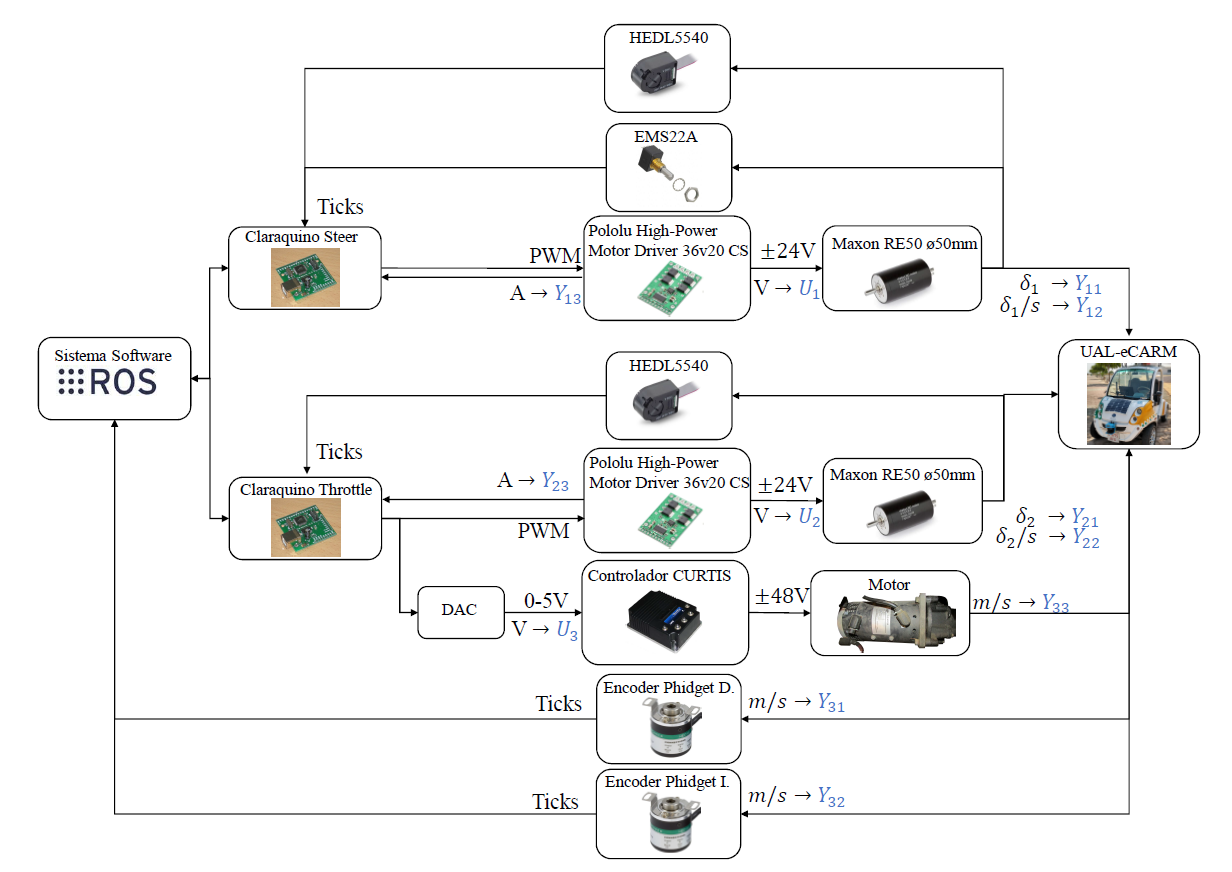
\includegraphics[width=1\textwidth]{Figuras/Diagrama_completo.PNG}
  \caption{Diagramas de bloques de la arquitectura hardware.}
  \label{fig:diagramas_bloques_hardware}
\end{figure}

\begin{figure}[!ht]
  \centering
    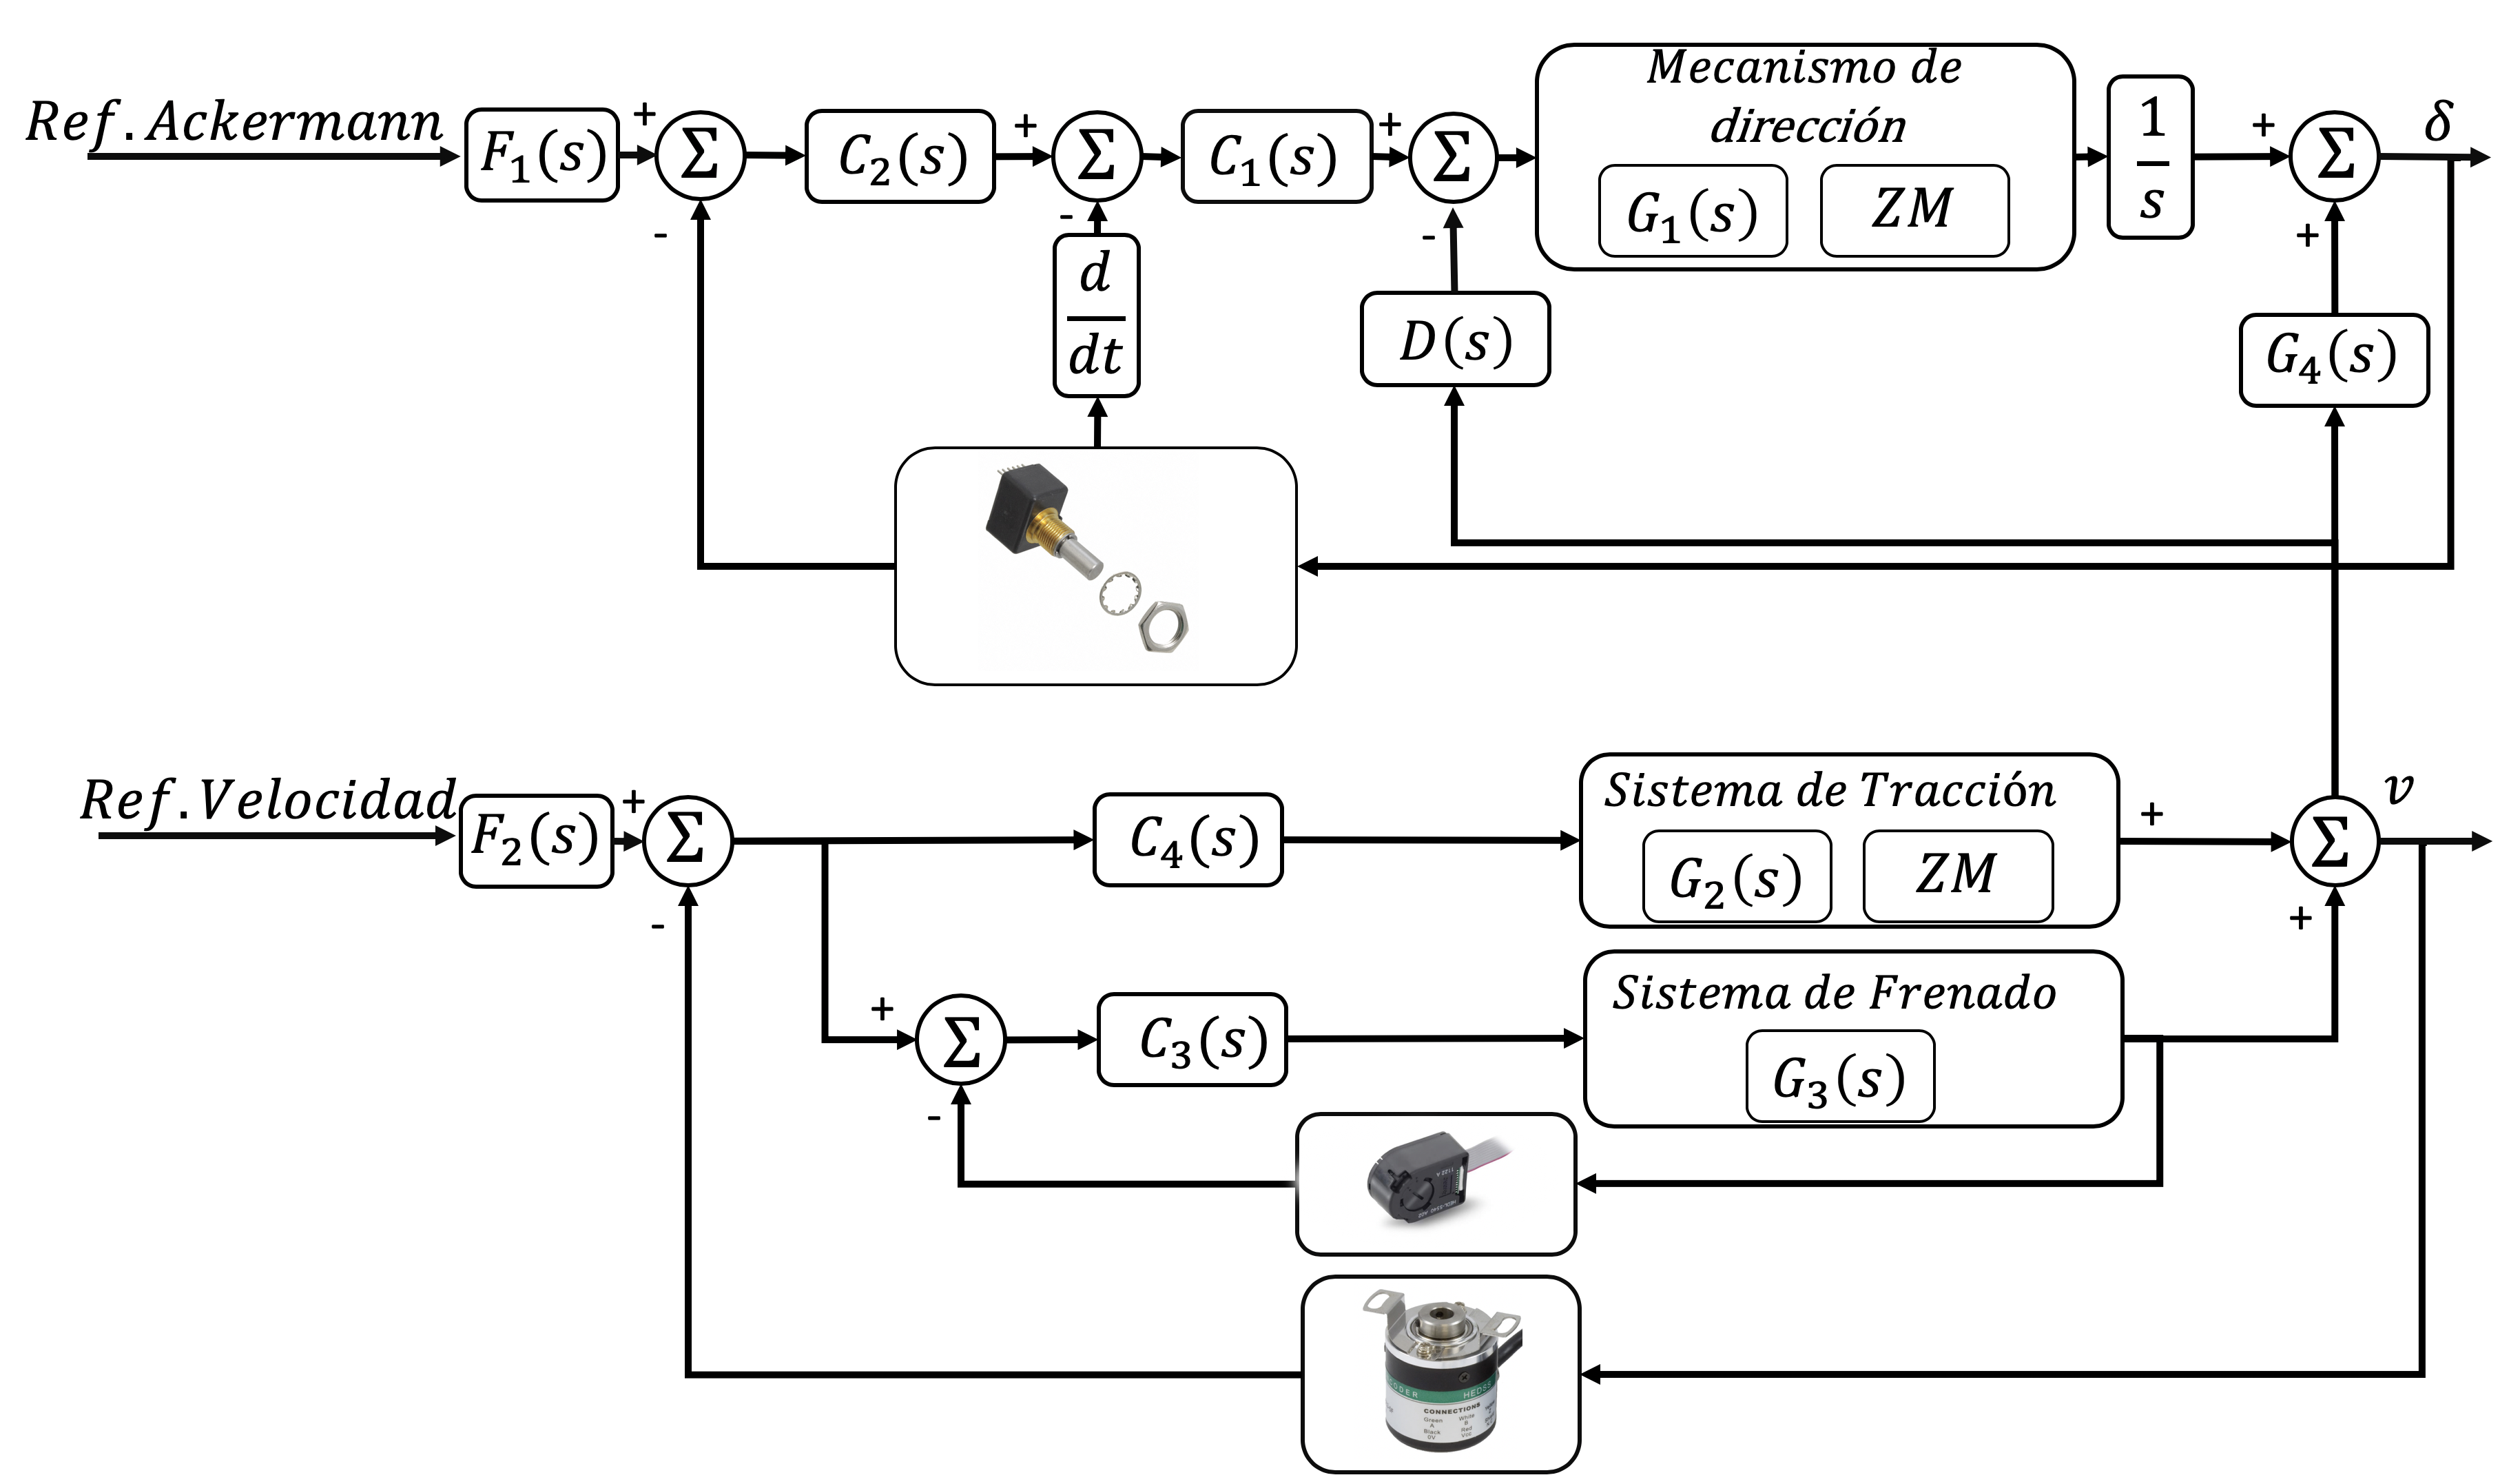
\includegraphics[width=1\textwidth]{Figuras/Diagrama_Bloques.PNG}
  \caption{Diagramas de bloques de las funciones de transferencia.}
  \label{fig:diagramas_bloques}
\end{figure}
% Revisión Bibliográfica
% Se podría realizar una búsqueda bibliográfica de artículos importantes.
% Capítulo 2. Historia/Revisión Bibliográfica
%%%%%%%%%%%%%%%%%%%%%%%%%%%%%%%%%%%%%%%%%%%%%%
% Todos los proyectos realizados sobre el vehículo
%%%%%%%%%%%%%%%%%%%%%%%%%%%%%%%%%%%%%%%%%%%%%%
\chapter{Trabajos anteriores}
\section{Trabajos Fin de Grado}
\textbf{Titulo:} \textit{Modelado del sistema de almacenamiento de energía y del controlador del motor para un vehículo eléctrico Tesur} \cite{kurucz2014Tesur}.

\textbf{Autor:} Kurucz , Adrian Paul.

\textbf{Director:} Rodríguez-Díaz, Francisco De Asís / Blanco-Claraco, José Luis.

\textbf{Grado:} Ingeniería Electrónica Industrial. \textbf{Curso:} 2013-14. 

\textbf{Ficha:} \url{http://repositorio.ual.es/handle/10835/3399}
 
\textbf{Resumen:} La situación energética actual y futura está condicionada por las limitadas reservas de combustibles fósiles, a lo que se suma la creciente preocupación por el medio ambiente y la eficiencia energética. Esta situación afecta especialmente al sector transportes, ya que es el mayor consumidor de energía. Los vehículos eléctricos se presentan como una solución prometedora a los problemas con los que se enfrenta el sector del transporte. Pero estos a su vez están condicionados por la energía eléctrica disponible a bordo, es decir, por el estado de carga de las baterías (SOC). Este parámetro no es medible, por lo cual es necesario estimarlo basándose en las mediciones de otras señales disponibles en las baterías, tales como tensión, corriente y temperatura. Este trabajo presenta un modelo eléctrico de las baterías, capaz de estimar el SOC, la tensión de las baterías y otros parámetros de interés a partir de la intensidad de descarga y la temperatura del electrólito de las baterías. Además, se ha realizado un estudio y análisis de tipos de baterías, centrándose en las baterías de Pb-ácido, sus características, modos de fallos, etc. La energía disponible a bordo se debe utilizar de forma eficiente, por ello en este trabajo también se procede a la caracterización del controlador del motor de impulsión de un vehículo eléctrico en función de las consignas de aceleración. 

%%%%%%%%%%%%%%%%%%%%%%%%%%%%%%%%%%%%%%%%%%%%%%%%%%%%%%%%%%%%%%%%%%%%%%%%%%%%%%%%%%%%%%%%%
\vspace{6pt} \hrule \vspace{6pt}
%%%%%%%%%%%%%%%%%%%%%%%%%%%%%%%%%%%%%%%%%%%%%%%%%%%%%%%%%%%%%%%%%%%%%%%%%%%%%%%%%%%%%%%%%
 
 \textbf{Titulo:} \textit{Modelado y control de la dirección de un vehículo eléctrico} \cite{ramos2014direccion}.

\textbf{Autor:} Ramos Teodoro, Jerónimo.

\textbf{Director:} Blanco-Claraco, José Luis / Rodríguez-Díaz, Francisco De Asís.

\textbf{Grado:} Ingeniería Mecánica. \textbf{Curso:} 2013-14. 

\textbf{Ficha:} \url{http://repositorio.ual.es/handle/10835/3408}
 
\textbf{Resumen:} En la actualidad, el uso creciente del automóvil unido al desarrollo de Sistemas Inteligentes de Transporte, fomenta la investigación en el ámbito de los vehículos autónomos. Este trabajo tiene por objetivo el diseño de un sistema para el control de bajo nivel de la dirección de un vehículo eléctrico, siguiendo un esquema en cascada para el control lateral del mismo. Para ello, se instalan y calibran los elementos de medición y actuación que permiten el control en lazo cerrado del ángulo de Ackermann, dado por la posición de las ruedas directrices del vehículo, y se elabora un modelo de diagrama de bloques con la herramienta Simulink de MATLAB que se ajusta al comportamiento del sistema. Una vez validado el modelo, se diseña e implementa el sistema adecuado para el control Proporcional Integral Derivativo de la posición angular y se somete a pruebas de funcionamiento en un entorno de simulación. La principal aportación, además de poder integrar el modelo construido en Simulink en un modelo global del vehículo, consiste en que proporciona la base para la aplicación de algoritmos de navegación autónoma sobre el vehículo.

%%%%%%%%%%%%%%%%%%%%%%%%%%%%%%%%%%%%%%%%%%%%%%%%%%%%%%%%%%%%%%%%%%%%%%%%%%%%%%%%%%%%%%%%%
\vspace{6pt} \hrule \vspace{6pt}
%%%%%%%%%%%%%%%%%%%%%%%%%%%%%%%%%%%%%%%%%%%%%%%%%%%%%%%%%%%%%%%%%%%%%%%%%%%%%%%%%%%%%%%%%

\textbf{Titulo:} \textit{Diseño y construcción de un banco de ensayo para la caracterización del motor de un vehículo eléctrico} \cite{acuna2014motor}.

\textbf{Autor:} Acuña-Prieto, Francisco.

\textbf{Director:} Giménez-Fernández, Antonio / Torres-Moreno, José Luis.

\textbf{Grado:} Ingeniería Mecánica. \textbf{Curso:} 2014-15.

\textbf{Resumen:} El sector del transporte ha aumentado su demanda en los últimos años y se ha convertido en el sector con mayor consumo de energía. Esto ha provocado que, actualmente, la industria se centre en desarrollar vehículos más fiables y respetuosos con el medio ambiente. Este proyecto tiene por objetivo el diseño y construcción de un banco de ensayo capaz de realizar las mediciones necesarias para la caracterización de un motor de un vehículo eléctrico. Para ello, se realiza un diseño CAD de los elementos que requiere el banco para su funcionamiento y se fabrica la estructura. Posteriormente, se replica el sistema eléctrico del vehículo para adaptarlo al banco, y se monta la instrumentación. Finalmente, se realizan algunos ajustes a la configuración del controlador del motor, se diseña un sistema de adquisición de datos y se realizan los ensayos. La principal aportación del proyecto, además de crear una herramienta que permita obtener los parámetros para realizar el control de un motor eléctrico, consiste en ofrecer la posibilidad de, realizando algunas modificaciones, simular diferentes situaciones que se encontraría el vehículo eléctrico en la realidad.
 
%%%%%%%%%%%%%%%%%%%%%%%%%%%%%%%%%%%%%%%%%%%%%%%%%%%%%%%%%%%%%%%%%%%%%%%%%%%%%%%%%%%%%%%%%
\vspace{6pt} \hrule \vspace{6pt}
%%%%%%%%%%%%%%%%%%%%%%%%%%%%%%%%%%%%%%%%%%%%%%%%%%%%%%%%%%%%%%%%%%%%%%%%%%%%%%%%%%%%%%%%%
 
\textbf{Titulo:} \textit{Análisis e instalación de un sistema fotovoltaico en el vehículo eléctrico UAL-eCARM} \cite{guerrero2015solar}.

\textbf{Autor:} Guerrero-Cabezas, Francisco Javier.

\textbf{Director:} Rodríguez-Díaz, Francisco De Asís.

\textbf{Grado:} Ingeniería Mecánica. \textbf{Curso:} 2015-16. 

%\textbf{Ficha:} \url{http://repositorio.ual.es/handle/}
 
\textbf{Resumen:} En la actualidad, el desarrollo de la tecnología, la reducción de costes en instalaciones y la concienciación social acerca de los problemas medioambientales han impulsado el interés por las fuentes de energía renovables cuya principal ventaja competitiva es su concepción como fuente inagotable. El objetivo de este trabajo es por lo tanto, el estudio de las características e instalación de un sistema fotovoltaico aislado como fuente de energía alternativa y/o complementaria a la red eléctrica en un vehículo eléctrico y el análisis de su eficiencia energética. Siendo así, se ha calculado y diseñado un equipo de medida para analizar un Sistema Fotovoltaico Aislado (SFA) en régimen de corriente continua, con objeto de estudiar las Curvas Tensión-Intensidad características. Posteriormente a los resultados de dicho estudio y con el conocimiento de las distintas condiciones que supeditan su funcionamiento, se ha llevado a cabo la instalación del SFA en el vehículo eléctrico y se ha dispuesto la instrumentación electrónica necesaria para llevar a cabo el estudio de los procesos de carga y descarga de los acumuladores presentes. La principal aportación ha consistido en facilitar el acceso al conocimiento de los factores determinantes en la eficiencia de un Sistema Fotovoltaico mediante el equipo diseñado y acotar un camino hacia la búsqueda de soluciones para dotar de mayor trascendencia a las ventajas propias de la energía solar fotovoltaica.
 
%%%%%%%%%%%%%%%%%%%%%%%%%%%%%%%%%%%%%%%%%%%%%%%%%%%%%%%%%%%%%%%%%%%%%%%%%%%%%%%%%%%%%%%%%
\vspace{6pt} \hrule \vspace{6pt}
%%%%%%%%%%%%%%%%%%%%%%%%%%%%%%%%%%%%%%%%%%%%%%%%%%%%%%%%%%%%%%%%%%%%%%%%%%%%%%%%%%%%%%%%% 

\textbf{Titulo:} \textit{Estudio de la dirección de un vehículo eléctrico mediante herramientas CAD-CAE} \cite{perez2017CAD}.

\textbf{Autor:} Pérez-Candela, Alberto José.

\textbf{Director:} Torres-Moreno, José Luis.

\textbf{Grado:} Ingeniería Mecánica. \textbf{Curso:} 2016-17. 

%\textbf{Ficha:} \url{http://repositorio.ual.es/handle/}
 
\textbf{Resumen:} El sector automovilístico es conocido como un sector con un gran potencial y rentabilidad. Esto unido a los crecientes avances en los Sistemas Inteligentes de Transporte, invita al desarrollo y el estudio de este nicho de oportunidades que se nos abre. Este proyecto tiene por objetivo la implementación de un sistema de control de la dirección y de la amortiguación del vehículo eléctrico de la UAL eCARM, conectando un modelo tridimensional a este, consiguiendo de este modo los parámetros de todo el sistema de dirección y reduciendo así el número de sensores que debería tener el vehículo. Para ello, primero se mide y modela en 3D con el programa SolidWorks respetando su posición original y aplicando las condiciones de contorno convenientes. En segundo lugar se combina dicho modelo con un sistema SCADA que permite conseguir información a partir del modelo además de realizar su control. Finalmente, la creación de un prototipo a base de actuadores y sensores que se comunican con el software y permite su control y la reducción del error mediante lo que se conoce como “Hardware in Loop” (HIL). La principal aportación es la integración el modelo 3D construido en SolidWorks con LabView para su cosimulación, lo que permite la reducción de sensores para el conocimiento de la posición y el control del sistema de dirección. Además de esta aportación, la otra aportación es la creación de un prototipo con las mismas dimensiones que el eCARM y que permita la simulación del movimiento de la dirección y la amortiguación.

%%%%%%%%%%%%%%%%%%%%%%%%%%%%%%%%%%%%%%%%%%%%%%%%%%%%%%%%%%%%%%%%%%%%%%%%%%%%%%%%%%%%%%%%%
\vspace{6pt} \hrule \vspace{6pt}
%%%%%%%%%%%%%%%%%%%%%%%%%%%%%%%%%%%%%%%%%%%%%%%%%%%%%%%%%%%%%%%%%%%%%%%%%%%%%%%%%%%%%%%%%

\textbf{Titulo:} \textit{Caracterización y control de sistema drive-by-wire en vehículo eléctrico}\cite{manas2017UALeCARM}.

\textbf{Autor:} Mañas-Álvarez, Francisco José.

\textbf{Director:} Blanco-Claraco, José Luis / Guzmán-Sánchez, José Luis.

\textbf{Grado:} Ingeniería Electrónica Industrial. \textbf{Curso:} 2016-17. 

\textbf{Ficha:} \url{http://repositorio.ual.es/handle/10835/6436}
 
\textbf{Resumen:} La elevada demanda de vehículos, el progreso tecnológico asociado a la automatización de nuestro entorno y la preocupación por la conservación del medio ambiente está guiando la investigación de vehículos hacia mejores resultados con vehículos eléctricos y autónomos. Pero el control a tan alto nivel no es posible si en los niveles inferiores, los sistemas de control no son lo suficientemente eficaces. Este trabajo presenta como objetivo la realización de un control eficaz a bajo nivel sobre los sistemas Steer-by-wire y Throttle-by-wire. Para ello, en primer lugar se debe realizar el modelado de los sistemas actuales del vehículo. Una vez se comprueba la validez de los modelos obtenidos, se trabaja en el diseño de los sistemas de control mediante herramientas de simulación, en este caso se emplea principalmente Simulink. Los principales problemas tratados en el trabajo son la identificación de modelos de alto orden, en el caso del sistema Throttle-by-wire, y el control en cascada con un sistema de retardo dominante en el lazo interno para el caso del sistema Steer-by-wire. Posteriormente, con el sistema de control ya diseñado y comprobada su eficiencia en simulación, se implementa en el sistema real incorporándolo al sistema ya existente creado en ROS. La principal aportación de este trabajo, además de la actualización de los modelos instalados en el vehículo eCARM, es la implementación del sistema de control completo en el nodo steer\_controller del sistema ROS.

%%%%%%%%%%%%%%%%%%%%%%%%%%%%%%%%%%%%%%%%%%%%%%%%%%%%%%%%%%%%%%%%%%%%%%%%%%%%%%%%%%%%%%%%%
\vspace{6pt} \hrule \vspace{6pt}
%%%%%%%%%%%%%%%%%%%%%%%%%%%%%%%%%%%%%%%%%%%%%%%%%%%%%%%%%%%%%%%%%%%%%%%%%%%%%%%%%%%%%%%%%
 
\textbf{Titulo:} \textit{Integración y caracterización del sistema fotovoltaico en el vehículo UAL-eCARM} \cite{poyatos2019UALeCARM}.

\textbf{Autor:} Poyatos Bakker, Aaron Raúl.

\textbf{Director:} Blanco-Claraco, José Luis / Torres-Moreno, José Luis.

\textbf{Grado:} Ingeniería Mecánica. \textbf{Curso:} 2018-19. 

%\textbf{Ficha:} \url{http://repositorio.ual.es/handle/}
 
\textbf{Resumen:} Hoy en día, la sociedad tiene cada vez m as presente el impacto negativo que producen al medioambiente los vehículos que emplean fuentes no renovables. Con el desarrollo de la tecnología y la optimización de las fuentes renovables, se abren las posibilidades de implementar sistemas de carga en vehículos eléctricos. El objetivo de este trabajo ha sido precisamente el estudio y la selección de los elementos necesarios para integrar un sistema fotovoltaico como fuente de energía aislada en un vehículo eléctrico; así como su lectura y transmisión de estados vía la red de comunicaciones que emplea el propio vehículo, a través del uso de un middleware robótico llamado ROS (Robot Operating System). Para ello se ha desarrollado un paquete específico en el entorno ROS, dedicado exclusivamente al filtrado e interpretación de los valores del sistema fotovoltaico y transmitir de manera automática aquellos valores de inter es (voltaje e intensidad del sistema de baterías y de los módulos fotovoltaicos). Posteriormente, se ha realizado la instalación en el vehículo de todos los componentes que integran el sistema fotovoltaico y se han llevado a cabo ensayos experimentales para el análisis energético del sistema. Este trabajo aporta una visión clara sobre el procedimiento de instalación de un sistema fotovoltaico en un vehículo eléctrico. Y describe la configuración necesaria dentro del entorno ROS, de cómo establecer una vía de comunicación con el regulador de carga: el
dispositivo encargado de controlar y estabilizar el sistema fotovoltaico.
 
\section{Trabajos Fin de Máster}
\textbf{Titulo:} \textit{Estudio del comportamiento dinámico de un vehículo eléctrico mediante SimMechanics} \cite{torres2011UALeCARM}.

\textbf{Autor:} Torres-Moreno, José Luis.

\textbf{Director:} Giménez-Fernández, Antonio.

\textbf{Máster:} Informática Industrial . \textbf{Curso:} 2010-11. 

\textbf{Ficha:} \url{http://hdl.handle.net/10835/1187}
 
\textbf{Resumen:} The introduction of electric propulsion systems in automobiles is helping to reduce fossil fuel consumption and optimize the e ciency of new vehicles. This paper analyzes and simulates the dynamic behavior of an electric vehicle. Dynamic equations are formulated and a three-dimensional prototype is built, which allows the collection of data on mass and inertia of its components. All these variables are implemented in a model that is analyzed by the tool for the analysis of Multibody systems SimMechanics. The main contribution of this paper is the proposal, once validated the model, of a change in the distribution of mass of the vehicle which improves the dynamic performance of it. And thanks to the integration of this model in MATLAB / Simulink, future additions such as navigation systems, autonomous control, brake assist and stability control, among others are possible.
 
%%%%%%%%%%%%%%%%%%%%%%%%%%%%%%%%%%%%%%%%%%%%%%%%%%%%%%%%%%%%%%%%%%%%%%%%%%%%%%%%%%%%%%%%%
\vspace{6pt} \hrule \vspace{6pt}
%%%%%%%%%%%%%%%%%%%%%%%%%%%%%%%%%%%%%%%%%%%%%%%%%%%%%%%%%%%%%%%%%%%%%%%%%%%%%%%%%%%%%%%%%

\textbf{Titulo:} \textit{Modelado y control multivariable del vehículo urbano eléctrico UAL-eCARM} \cite{manas2019UALeCARM}.

\textbf{Autor:} Mañas-Álvarez, Francisco José.

\textbf{Director:} Blanco-Claraco, José Luis / Rodríguez-Díaz, Francisco De Asís.

\textbf{Grado:} Ingeniería Industrial. \textbf{Curso:} 2018-19. 

%\textbf{Ficha:} \url{http://repositorio.ual.es/handle/}
 
\textbf{Resumen:} Los sistemas de gran complejidad, como los vehículos, necesitan que todos sus elementos funcionen bien tanto de forma individual como en conjunto. Si la sinergia entre los distintos subsistemas es elevada, mejor es el desempeño de los resultados obtenidos. Este trabajo presenta como objetivo la mejora de la plataforma UAL-eCARM, un vehículo eléctrico urbano. El trabajo comprende el modelado y control de los sistemas de dirección y tracción del vehículo. Para ello se han mejorado los modelos y arquitecturas de control del mecanismo Steer-by-Wire. El sistema Throttle-by-Wire, un sistema no lineal, ha sido modelado como un sistema lineal entorno a cuatro puntos de operación. La estrategia de control implementada es un controlador PI adaptativo según el ajuste de Ziegler-Nichols. El sistema Brake-by-Wire, el más reciente instalado, se ha modelado y controlado mediante un controlador PI ajustado manualmente. La implementación está disponible en Github. Las principales aportaciones de este trabajo son la ampliación y mejora de los modelos del vehículo UAL-eCARM y la migración de la arquitectura de control desde los nodos de ROS a
microcontroladores.
 
\section{Doctorados}
\textbf{Titulo:} \textit{Análisis multidominio de vehículos eléctricos} \cite{torres2014UALeCARM}.

\textbf{Autor:} Torres-Moreno, José Luis.

\textbf{Director:} Giménez-Fernández, Antonio / Blanco-Claraco, José Luis.

\textbf{Doctorado:} En Informática. \textbf{Año:} 2014. 
 
\textbf{Resumen:} El automóvil es uno de los productos tecnológicos consumidos a gran escala que abarca un mayor número de sistemas mecánicos, eléctricos y electrónicos. Todos estos sistemas son complejos y afectan de forma individual o interactuando entre ellos al funcionamiento del vehículo en su conjunto. Además, el número de sistemas de control que incorporan los coches modernos cada vez es mayor. Para poder diseñar un controlador es preciso conocer en primer lugar cómo se comportan los sistemas que determinan el funcionamiento del vehículo. Desde esta tesis se proponen una serie de metodologías para analizar dichos sistemas. Estas metodologías son muy diferentes dependiendo del sistema del automóvil que se estudie. Por tanto se analizará cada una de ellas por separado.

Dada la inminente aparición masiva de vehículos con motores diferentes de los de combustión interna (en combinación con éstos o sustituyéndolos), se hace necesario un estudio de este tipo de vehículos. Entre las opciones más destacadas se encuentran los denominados vehículos híbridos eléctricos, cuyas particularidades implican atender a aspectos que no estaban presentes en los vehículos convencionales, como puede ser el control de un sistema de propulsión totalmente renovado o el comportamiento dinámico derivado de una distribución de masas diferente a la de los vehículos de gasolina. Algunas de las metodologías propuestas en esta tesis están orientadas a analizar estas características, incluyendo el diseño de una estrategia de control de gestión energética para la utilización conjunta de las diferentes fuentes de potencia incorporadas en vehículos híbridos eléctricos.

En las fases tempranas del diseño de un vehículo se prefiere, en la medida de lo posible, trabajar con modelos en lugar de con prototipos físicos. Por este motivo, en esta tesis se exploran varias alternativas que permitan la realización de experimentos mediante simulaciones. Entre los modelos considerados aparecen, por un lado, los modelos multicuerpo, que pueden alcanzar un alto nivel de realismo, y los modelos simplificados, ideales para diseñar controladores y observadores de estado. Esto no exime de la necesidad de realizar experimentos reales con un prototipo. Este, deberá de incorporar una serie de sensores y actuadores que permitan medir los parámetros que mejor definen el su comportamiento. Además es necesario contar con una arquitectura de control que se encargue de gestionar las comunicaciones que tienen lugar en las diferentes capas. En esta tesis también se presenta la metodología llevada a cabo para la construcción de una arquitectura que proporciona una capa de abstracción en el vehículo que facilita la implementación de algoritmos de control.
 
\section{Artículos}
\textbf{Titulo:} \textit{Benchmarking Particle Filter Algorithms for Efficient Velodyne-Based Vehicle Localization} \cite{blanco2019benchmarking}.

\textbf{Autores:} Blanco-Claraco, J. L., Mañas-Alvarez, F., Torres-Moreno, J. L., Rodriguez, F., y Gimenez-Fernandez, A.

\textbf{Revista:} Sensors 2019, 19(14), 3155; \url{https://doi.org/10.3390/s19143155}

\textbf{Resumen:} Keeping a vehicle well-localized within a prebuilt-map is at the core of any autonomous vehicle navigation system. In this work, we show that both standard SIR sampling and rejection-based optimal sampling are suitable for efficient (10 to 20 ms) real-time pose tracking without feature detection that is using raw point clouds from a 3D LiDAR. Motivated by the large amount of information captured by these sensors, we perform a systematic statistical analysis of how many points are actually required to reach an optimal ratio between efficiency and positioning accuracy. Furthermore, initialization from adverse conditions, e.g., poor GPS signal in urban canyons, we also identify the optimal particle filter settings required to ensure convergence. Our findings include that a decimation factor between 100 and 200 on incoming point clouds provides a large savings in computational cost with a negligible loss in localization accuracy for a VLP-16 scanner. Furthermore, an initial density of aprox. 2 particles/m 2 is required to achieve 100\% convergence success for large-scale (aprox. 100,000 m 2 ), outdoor global localization without any additional hint from GPS or magnetic field sensors. All implementations have been released as open-source software.

%%%%%%%%%%%%%%%%%%%%%%%%%%%%%%%%%%%%%%%%%%%%%%%%%%%%%%%%%%%%%%%%%%%%%%%%%%%%%%%%%%%%%%%%%
\vspace{6pt} \hrule \vspace{6pt}
%%%%%%%%%%%%%%%%%%%%%%%%%%%%%%%%%%%%%%%%%%%%%%%%%%%%%%%%%%%%%%%%%%%%%%%%%%%%%%%%%%%%%%%%%

\textbf{Titulo:} \textit{Modelado y control multivariable del vehículo urbano eléctrico UAL-eCARM}\cite{manas2020byWire}.

\textbf{Autores:} Mañas-Álvarez, F.J., JBlanco-Claraco, J. L., Torres-Moreno, J. L. y Gimenez-Fernandez, A.

\textbf{Revista:} Revista Iberoamericana de Automática e Informática Industrial 2020, ??(??), ????; \url{https://doi.org/10.4995/riai.2019.12679}

\textbf{Resumen:}Este trabajo presenta el modelado y control completo del sistema Drive-by-Wire de un vehículo urbano eléctrico. Dicho sistema comprende el mecanismo de dirección, la aceleración y el freno del vehículo. El modelado se ha realizado empleando funciones de transferencia de bajo orden haciendo uso de modelos de “caja negra”. En lo referente al control, todos los controladores desarrollados son del tipo PID en sus distintas configuraciones. Los actuadores de corriente continua acoplados a la dirección y freno se controlan mediante un sistema de control en cascada mientras que la aceleración está controlada por un sistema de planificación de ganancias. El código del proyecto se encuentra disponible en la plataforma Github. Los resultados obtenidos demuestran la validez de los modelos obtenidos, así como la eficacia de los controladores desarrollados.

\section{Congresos}
\textbf{Titulo:} \textit{Caracterización y control del sistema Steer-By-Wire en un vehículo eléctrico}\cite{manas2019CIBIM}.

\textbf{Autores:} Mañas-Álvarez, Francisco José, López-Velasquez, Julián, Blanco-Claraco, José Luis, Torres-Moreno, José Luis, Giménez-Fernández, Antonio y Acosta-Amaya, Gustavo Alonso.

\textbf{Congreso:} 14 Congreso Iberoamericano de Ingeniería Mecánica.

\textbf{Localización:} Cartagena, Colombia. \textbf{Año:} 2019. 

\textbf{Resumen:} En este trabajo se afronta la realización de un control eficaz a bajo nivel sobre el sistema Steer-by-wire del prototipo de vehículo eléctrico autónomo desarrollado en la Universidad de Almería. En primer lugar, se obtiene la dinámica del motor DC encargado de actuar sobre la cremallera de dirección. Obteniendo un modelo de primer orden con retardo dominante para el comportamiento de la velocidad de giro del motor, se plantea un sistema de control en cascada para el control de la posición. Los posibles errores por saturación de la señal de control se evitan gracias a la implementación de la estrategia anti-windup a ambos controladores. Para facilitar la labor de validación de modelos y ensayo del sistema de control a instalar, se ha trabajado en simulación con la herramienta Simulink. El vehículo experimental está dotado con un PC industrial, y las aplicaciones corren bajo Ubuntu y ROS. La implementación se ha realizado mediante un nodo ROS que soporta el algoritmo de control y se comunica con la arquitectura hardware. En vista de los resultados obtenidos, la arquitectura de control ha demostrado ser robusta.

\afterpage{\blankpage}
% Capítulo 3. Componentes del vehículo
%%%%%%%%%%%%%%%%%%%%%%%%%%%%%%%%%%%%%%%%%%%%%%
% Descripción completa del vehículo
%%%%%%%%%%%%%%%%%%%%%%%%%%%%%%%%%%%%%%%%%%%%%%
\chapter{Componentes del vehículo}
Las características técnicas del vehículo a nivel constructivo se pueden encontrar en la página web del fabricante \cite{Greenland} (\textit{Changzhou Greenland Vehicle Co., Ltd,}) y se muestran en la tabla \ref{Tab:medidas_UALeCARM} para facilitar la labor.

\begin{table}[H]
\caption{Características técnicas del vehículo \textit{UAL-eCARM}.}\label{Tab:medidas_UALeCARM}
\centering
\begin{tabular}{|c |c |c |c|}
\hline % inserts single horizontal line
Parámetro & Medida & Parámetro & Medida \\
\hline
Longitud & 2680 mm  &  Velocidad máxima &  45km/h  \\
\hline
Anchura &  1510 mm  & Autonomía & 90 km \\
\hline
Altura & 1780 mm  & Radio de giro mínimo & 4.3 m \\
\hline
Distancia entre ejes &  1830 mm  & Peso & 740 kg \\
\hline
Paso ruedas traseras & 1285 mm  & Peso sin baterías &  460 kg \\
\hline
Paso ruedas delanteras & 1260 mm  &  Peso máximo &  950 kg \\
\hline
Pendiente máxima &  20\% &  Potencia máxima & 4.3 kW \\
\hline
\end{tabular}
\end{table}

\section{Energía}
La fuente de energía que posee el vehículo son 8 baterías de gel electrolítico de ácido-plomo reguladas por válvula (VRLA) marca Trojan, Figura \ref{fig:Bateria}. Anteriormente se disponía de 8 baterías de la marca \textit{Greensaver} modelo \textit{SP210-6}, Figura \ref{fig:Bateria-ant}. Para acceder a ellas se debe levantar la parte inferior de los asientos del vehículo, Figura \ref{fig:baterias-asientos}. Estas baterías suministran una tensión de 6 Voltios (V) y poseen una capacidad de 189 Amperio-hora (Ah). Con estas características, su conexión se produce en serie obteniendo una tensión total para distribuir en el vehículo de 48V. A pesar de que la tensión suministrada es de 48V, se considera necesario el empleo de conversores DC-DC que suministren líneas de tensión a 5V, 12V y 24V, puesto que no todos los dispositivos electrónicos que incorpora el vehículo trabajan a igual tensión.

\begin{figure}[h!]
\begin{center}
	\subfloat[Trojan 6V-GEL.]{
		\label{fig:Bateria}
		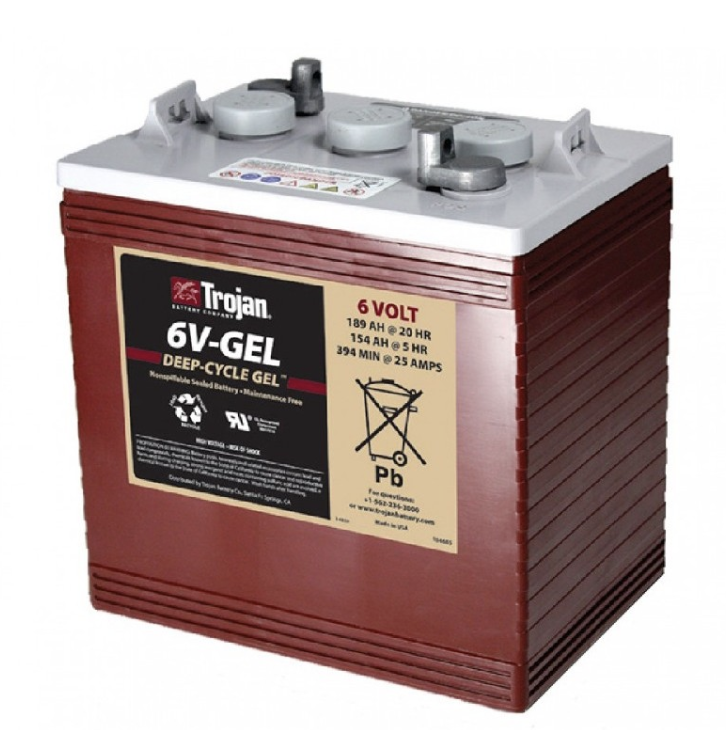
\includegraphics[width=0.35\textwidth]{Figuras/C3-Bateria}}
	\subfloat[Greensaver SP210-6.]{
		\label{fig:Bateria-ant}
		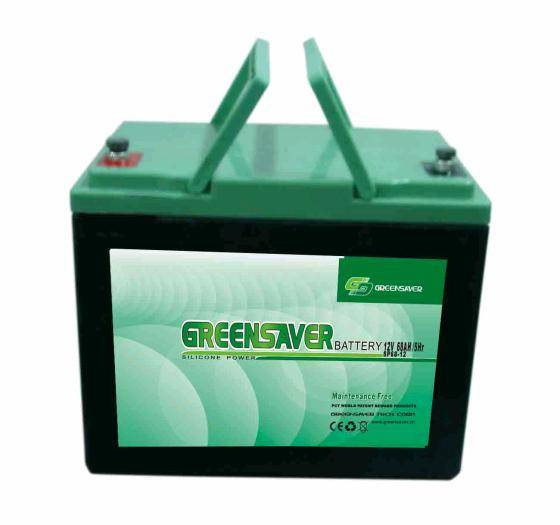
\includegraphics[width=0.4\textwidth]{Figuras/C3-Bateria-ant}}
	\caption{Baterías instaladas en el vehículo.}
\end{center}
\end{figure}

\begin{figure}[h!]
  \centering
    \includegraphics[width=1\textwidth]{Figuras/C3-Baterias-instalacion}
  \caption{Ubicación de las baterías en el vehículo.}
  \label{fig:baterias-asientos}
\end{figure}

\subsection{PowerBox}
Este componente, Figura \ref{fig:PowerBox}, presenta tres funciones principales:
\begin{itemize}
\item Proteger la instalación electrónica mediante la instalación previa de un fusible de 20A.

\item Encender los distintos componentes de forma individual o en pequeñas agrupaciones que permite evitar consumo innecesario de componentes que no se usan.

\item Cortar la alimentación de distintos elementos para manipularlos sin tener que apagar el vehículo entero.
\end{itemize}

A esta caja están conectadas las dos fuentes CC-CC, los dos reguladores y el PC industrial. Como protección principal se emplea un fusible de 20A a la entrada y un display que monitoriza la tensión, intensidad y consumo de todos los componentes conectados. Además se han implementado cinco interruptores que modularizan el encendido de cada componente y uno de ellos actúa como interruptor principal. Esto permite cierto nivel de ahorro energético que se produciría por el encendido de componentes que no se empleen en dicho momento y el encendido de componentes de forma individual para realizar ensayos sobre ellos.  

\subsection{Fuentes de alimentación}
Las baterías, como ya se comentó en la introducción de esta sección, suministran una tensión de 48V, pero no todos los dispositivos requieren dicha tensión. Para el establecimiento de las distintas tensiones requeridas se han empleado dos fuentes CC-CC las cuales convierten de 48V a 12V y 24V respectivamente y dos reguladores conmutados de 5V y 19V respectivamente. 

La fuente CC-CC de 24V, SD-500L-24 mean well (ver figura \ref{fig:FuenteDC}), se emplea para la alimentación del motor de la dirección, de los distintos amperímetros de la marca LEM situados por el vehículo (Baterías y motor) y el sensor láser de la parte frontal. La fuente de 12V, reutilizada de otros proyectos realizados anteriormente, suministra corriente al amperímetro Honeywell que cuantifica la corriente suministrada por las baterías. El regulador de 5V localizado en la caja denominada \textit{PowerBox} se emplea para la alimentación de aquella electrónica que opera a dicho nivel. El regulador de 19V se requiere para el funcionamiento del monitor situado en la cabina del vehículo. Para su correcto funcionamiento, puesto que el dispositivo integrado abarca un rango de tensiones de salida de 11.85V-22V, se construye un circuito físico para adecuar la tensión a 19V, figura \ref{fig:Regulador}.

\begin{figure}[h!]
\begin{center}
	\subfloat[Fuente CC-CC.]{
		\label{fig:FuenteDC}
		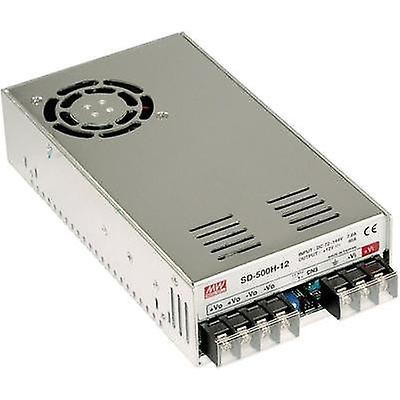
\includegraphics[width=0.3\textwidth]{Figuras/C3-DCDC}}
	\subfloat[Regulador.]{
		\label{fig:Regulador}
		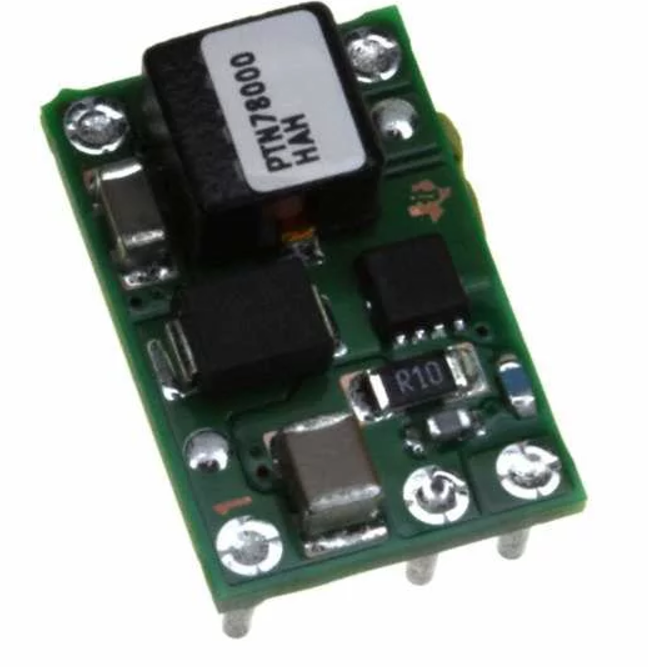
\includegraphics[width=0.3\textwidth]{Figuras/C3-Regulador}}
	\subfloat[PowerBox.]{
		\label{fig:PowerBox}
		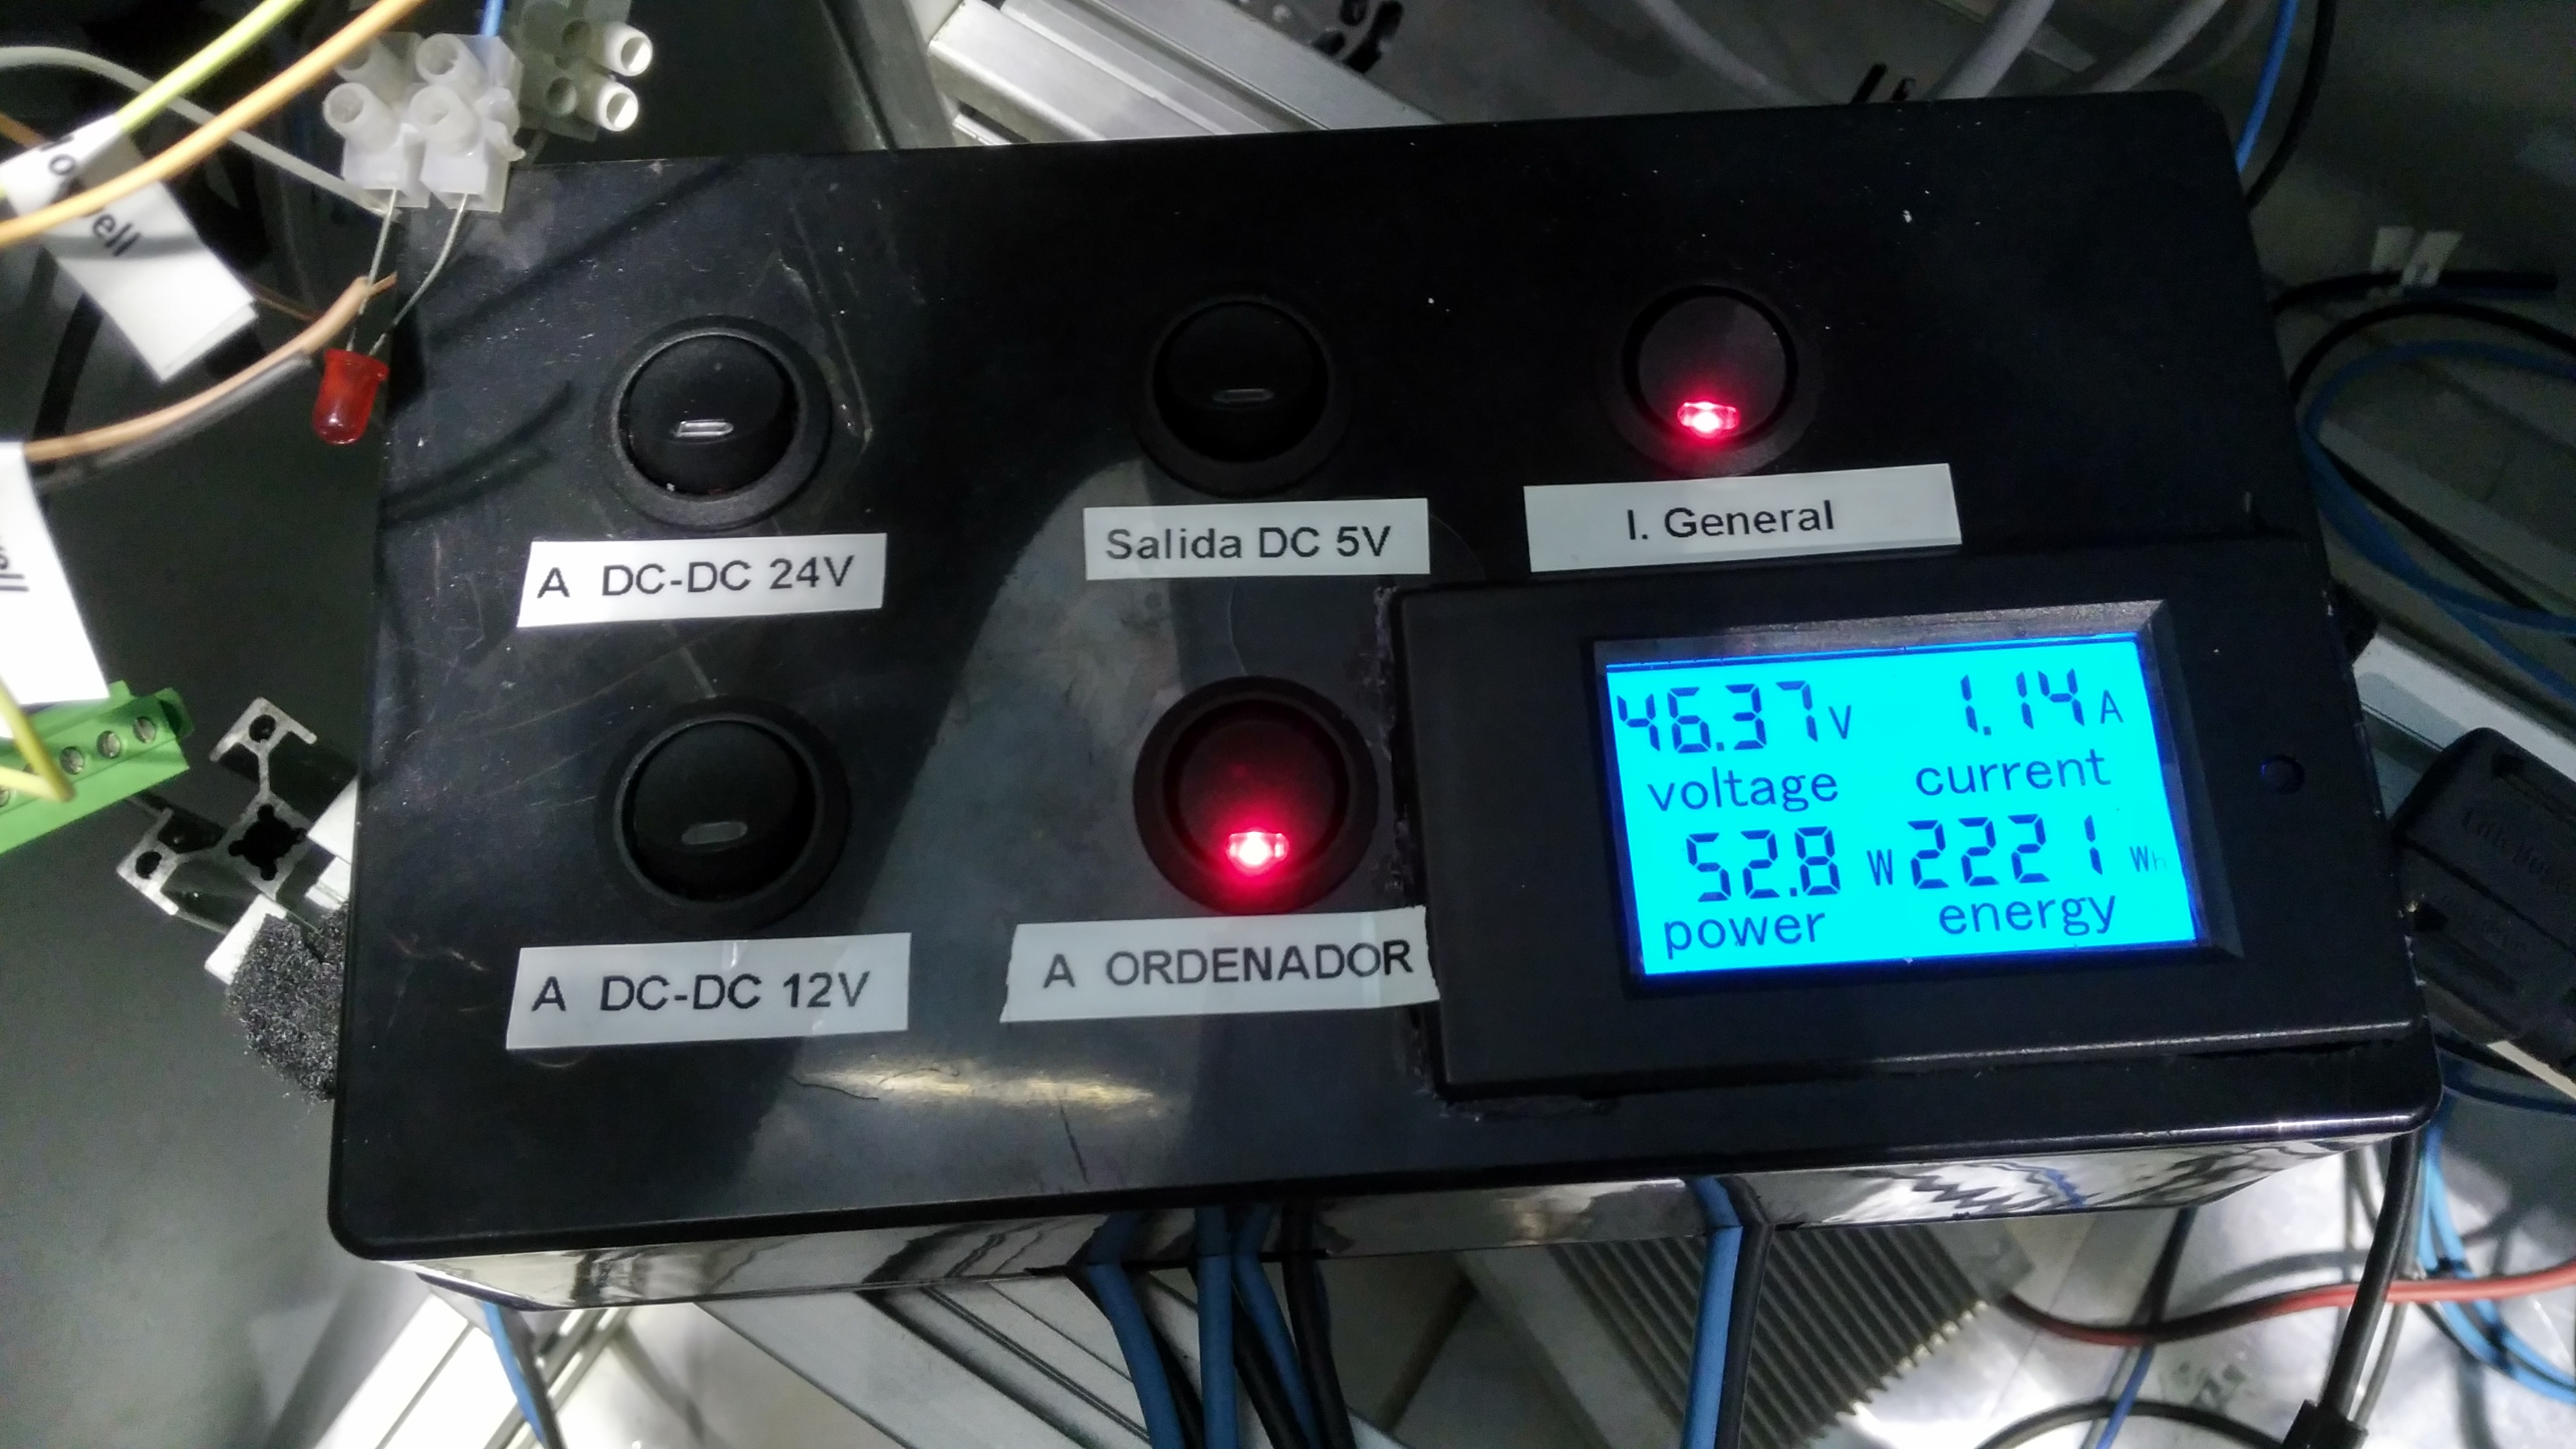
\includegraphics[width=0.35\textwidth]{Figuras/C3-PowerBox}}
	\caption{Componentes encargados de la administración de corriente.}
\end{center}
\end{figure}

\textbf{HAY QUE AÑADIR UN ESQUEMA QUE MUESTRE EL CABLEADO ELÉCTRICO DE LA ALIMENTACIÓN DEL VEHÍCULO}

\section{Tracción}

\section{Dirección}

\section{Otros sensores}


Describir TODO lo que hay instalado en el vehículo. Descripción completa y muy detallada de todos los componentes, características, hojas de fabricantes, que variables generan, si están estandarizadas o no, como se comunican con ROS, ... Incluir comentarios en cursiva con las apreciaciones de los que estén trabajando con ellos, como pequeños trucos o imperfecciones que haya que considerar y aún no se sepa porqué aparecen.

\section{Tareas Pendientes}
Cosas a instalar o calibrar.
% Capítulo 4. Firmware
%%%%%%%%%%%%%%%%%%%%%%%%%%%%%%%%%%%%%%%%%%%%%%
% Firmware
%%%%%%%%%%%%%%%%%%%%%%%%%%%%%%%%%%%%%%%%%%%%%%
\chapter{Firmware}

\afterpage{\blankpage}
% Capítulo 5. ROS
%%%%%%%%%%%%%%%%%%%%%%%%%%%%%%%%%%%%%%%%%%%%%%
%ROS
%%%%%%%%%%%%%%%%%%%%%%%%%%%%%%%%%%%%%%%%%%%%%%
\chapter{Robot Operating System}
Hablar sobre la estructura de ROS, no hace falta que sea muy detallado el aspecto genérico de ROS. Debe ser suficiente para manejarse con el coche y entender completamente como está estructurado el coche.
\afterpage{\blankpage}
% Capítulo 6. Sistema de dirección
%%%%%%%%%%%%%%%%%%%%%%%%%%%%%%%%%%%%%%%%%%%%%%
% Sistema de dirección
%%%%%%%%%%%%%%%%%%%%%%%%%%%%%%%%%%%%%%%%%%%%%%
\chapter{Sistema de dirección}
Establecer todo el contexto físico del mecanismo de dirección (ecuaciones) sin considerar aproximaciones. ACKERMANN. Las aproximaciones se pueden indicar a posteriori. Leyendo esta sección, se debe ser un experto en este mecanismo.

Realizar la identificación por todos los métodos posibles y comparar los resultados obtenidos: Caja negra, primeros principios; funciones de transferencia, espacios de estados; ... Pros y contras de cada una. Disponer de todos los modelos.

Estudiar los distintos sensores que dan información y aplicar Kalman para obtener la mejor salida o algo así. Estudiar desde el punto de vista energético también.
\afterpage{\blankpage}
% Capítulo 7. Sistema de tracción
%%%%%%%%%%%%%%%%%%%%%%%%%%%%%%%%%%%%%%%%%%%%%%
% Sistema de velocidad longitudinal
%%%%%%%%%%%%%%%%%%%%%%%%%%%%%%%%%%%%%%%%%%%%%%
\chapter{Movimiento longitudinal}
Realizar un análisis detallado de las ecuaciones que rigen la dinámica del vehículo. Estudiar a fondo el Curtis y establecer cual es la configuración más óptima de forma razonada y justificada. Leyendo esta se debe poder manipular el vehículo sin problemas y ser un experto en el asunto.

Al igual que en la dirección se debe realizar la identificación completa y comparativa del vehículo. Estudiar también desde el punto de vista energético.
\afterpage{\blankpage}
% Capítulo 8. Simuladores
%%%%%%%%%%%%%%%%%%%%%%%%%%%%%%%%%%%%%%%%%%%%%%
% Crear herramientas de simulación
%%%%%%%%%%%%%%%%%%%%%%%%%%%%%%%%%%%%%%%%%%%%%%
\chapter{Simuladores}
Crear herramientas de simulación para distintos entornos que permitan estudiar el vehículo offline.
\afterpage{\blankpage}
% Capítulo 9. Arquitectura de control
%%%%%%%%%%%%%%%%%%%%%%%%%%%%%%%%%%%%%%%%%%%%%%
% Arquitectura de control
%%%%%%%%%%%%%%%%%%%%%%%%%%%%%%%%%%%%%%%%%%%%%%
\chapter{Arquitectura de control}
Probad todas las estrategias de control posibles y generar el máximo de papers y congresos. Hay que sacarle rendimiento al coche. Aquí se realizaría un estudio detallado en simulación y experimental de cada estrategia para cada sistema.
\afterpage{\blankpage}

\bibliographystyle{ieeetr}
\bibliography{Bibliografia}

\end{document}
